\section{Diagnóstico de correlación cruzada}
\label{sec:correlación}

%\todo{Pregunta aca: vale la pena hacer el analisis para cada sujeto?}

La presencia de correlación entre los predictores de un modelo 
de regresión puede inflar la varianza de los coeficientes estimados 
y dificultar su interpretación. Si bien la regresión Ridge mitiga 
este problema mediante la penalización $\lambda \|\beta\|^2$, que 
estabiliza los coeficientes en presencia de predictores correlacionados, 
no lo elimina completamente. Por esta 
razón, se realiza un diagnóstico de correlación previo al modelado 
de EEG, con el objetivo de identificar pares redundantes y fundamentar 
decisiones de descarte antes de incorporar las variables al modelo.

Dado que varias variables presentan distribuciones fuertemente sesgadas, 
como se documentó en el análisis distribucional 
(sección~\ref{sec:analisis_distribucional}), se empleó la correlación 
de Spearman en lugar de la de Pearson. La correlación de Spearman opera 
sobre los rangos de los datos y es robusta a outliers y a la no 
normalidad, lo que la hace más apropiada para el conjunto de variables 
analizado.

La Figura~\ref{fig:heatmap_correlaciones} presenta la matriz de 
correlaciones de Spearman entre las 20 variables candidatas, calculada 
sobre el pool completo de fijaciones ($N = 61.252$). Los colores rojos 
indican correlaciones positivas y los azules correlaciones negativas; 
las etiquetas de cada variable están coloreadas según su grupo de 
pertenencia.

\begin{figure}[H]
    \centering
    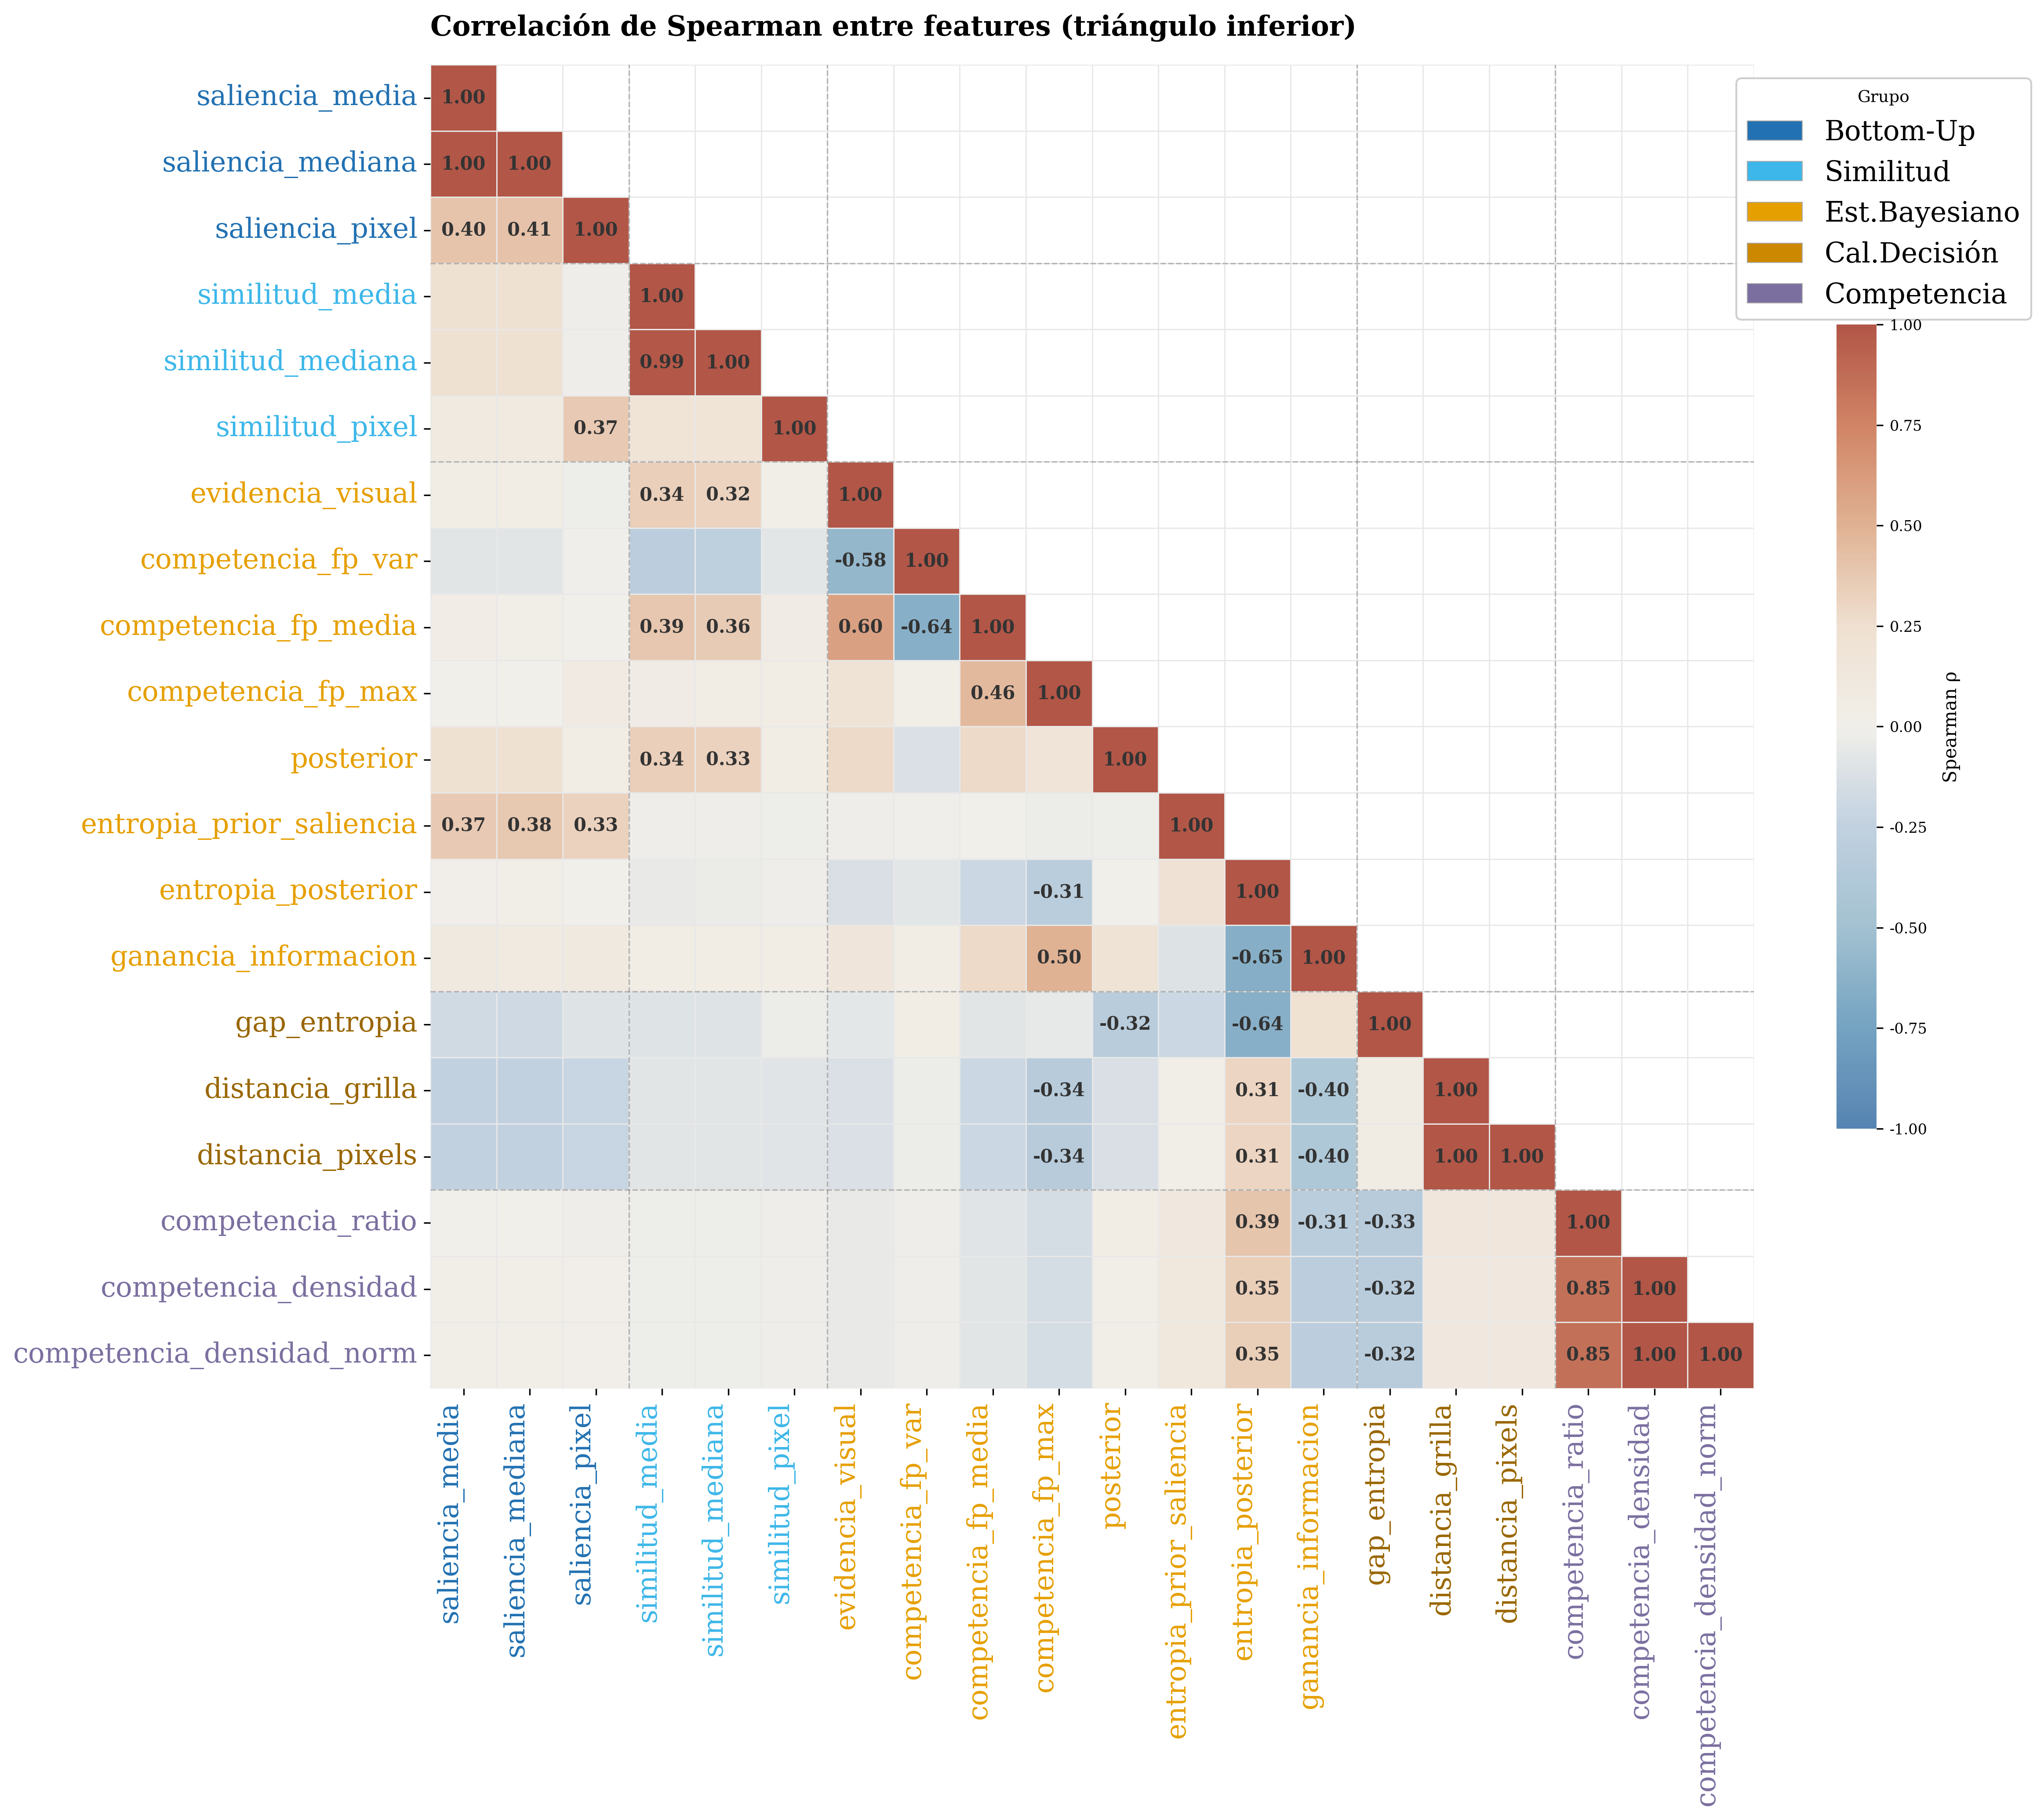
\includegraphics[width=\textwidth]{chapters/04_extraccion_analisis_variables/images/bloque5_corr_heatmap}
    \caption{Matriz de correlaciones de Spearman entre las variables 
    candidatas. Los colores de las etiquetas indican el grupo de 
    pertenencia de cada variable. Solo se muestran valores con $|\rho| \geq 0.30$}
    \label{fig:heatmap_correlaciones}
\end{figure}

\begin{sloppypar}
Se observan bloques de alta correlación
intragrupo en Bottom-Up y Similitud: \feat{saliencia\_media} y
\feat{saliencia\_mediana} presentan $\rho = 1.00$, y
\feat{similitud\_media} y \feat{similitud\_mediana} presentan
$\rho = 0.99$. Estas correlaciones son esperables dado que ambas
variables de cada par fueron diseñadas como resúmenes alternativos
de la misma información espacial y se incluyeron por separado
con el objetivo de evaluar su performance individual en el modelo.
Lo mismo ocurre dentro del grupo de Competencia:
\feat{competencia\_densidad} y \feat{competencia\_densidad\_norm}
presentan $\rho = 1.00$ por ser transformaciones lineales entre sí,
y ambas muestran una correlación moderada con
\feat{competencia\_ratio} ($\rho = 0.85$), también esperable dado
que las tres cuantifican distintos aspectos de la misma estructura
del mapa EIG.
\end{sloppypar}

En segundo lugar, se observan correlaciones altas entre grupos que 
no fueron anticipadas en el diseño de las variables. 
\feat{entropia\_posterior} y \feat{gap\_entropia} presentan 
una correlación negativa de $\rho = -0.79$, y 
\feat{ganancia\_informacion} y \feat{gap\_entropia} presentan 
una correlación positiva de $\rho = 0.69$. 

